% Clean CV/Resume Template, by Bennet B <dev@bennet.cc>
% CC0, Public-Domain
% 
% Permission is hereby granted, free of charge, to any person obtaining a copy
% of this template and associated files (the "Template"), to deal
% in the Template without restriction, including without limitation the rights
% to use, copy, modify, merge, publish, distribute, sublicense, and/or sell
% copies of the Template, and to permit persons to whom the Template is
% furnished to do so, subject to the following conditions:
%
% The above copyright notice and this permission notice shall be included in all
% copies or substantial portions of the Template.
%
% THE TEMPLATE IS PROVIDED "AS IS", WITHOUT WARRANTY OF ANY KIND, EXPRESS OR
% IMPLIED, INCLUDING BUT NOT LIMITED TO THE WARRANTIES OF MERCHANTABILITY,
% FITNESS FOR A PARTICULAR PURPOSE AND NONINFRINGEMENT. IN NO EVENT SHALL THE
% AUTHORS OR COPYRIGHT HOLDERS BE LIABLE FOR ANY CLAIM, DAMAGES OR OTHER
% LIABILITY, WHETHER IN AN ACTION OF CONTRACT, TORT OR OTHERWISE, ARISING FROM,
% OUT OF OR IN CONNECTION WITH THE TEMPLATE OR THE USE OR OTHER DEALINGS IN THE
% TEMPLATE.
%
% based on Modern CV by Habib Semouma
% https://www.overleaf.com/latex/templates/modern-cv-slash-resume-template/vjrqdkpjckwj
%
% 
\documentclass[oneside]{article}

\usepackage{wallpaper}
\usepackage{geometry}
\usepackage[
    unicode=true,
    bookmarks=true,
    bookmarksnumbered=false,
    bookmarksopen=true,
    bookmarksopenlevel=1,
    breaklinks=false,
    pdfborder={0 0 0},
    backref=false,
    colorlinks=false
    ]{hyperref}
\usepackage{lastpage}
\usepackage{hyphenat}
\usepackage{hyphsubst}
\usepackage{tabularx}
\usepackage{moresize}
\usepackage[document]{ragged2e}
% \usepackage{parskip}

\usepackage[scaled]{helvet}
\usepackage{fontawesome5}
\usepackage[defaultfam,tabular,oldstyle]{montserrat}
\usepackage[T1]{fontenc}
\renewcommand*\oldstylenums[1]{{\fontfamily{Montserrat-TOsF}\selectfont #1}}

\usepackage{titlesec}
\usepackage{xcolor}
\usepackage{graphicx}
\usepackage{tikz}

\setlength{\parindent}{0pt}
\titleformat{\section}{\normalfont}{}{0pt}{}

\renewcommand{\arraystretch}{1.4}

\setlength\fboxrule{0pt}
\setlength\fboxsep{12pt}
% \setlength{\parskip}{.5\baselineskip plus 2pt}
% \renewcommand{\baselinestretch}{1.1}

\titlespacing{\section}{0pt}{1.5ex plus .1ex minus .2ex}{1pc}

\newcolumntype{Y}{>{\RaggedRight\arraybackslash}X}

% Change PDF Meta Info here
\hypersetup{
    pdftitle={Qi Li - CV - English},
    pdfauthor={Qi Li},
    pdfsubject={Academic CV}
}

% Paper size
\geometry{
    a4paper,
    left=0pt,
    right=0pt,
    top=0pt,
    bottom=0pt,
    nohead,
    % includefoot,
    nomarginpar
}

% Background Color of the Sidebar Column - Tsinghua Purple
\definecolor{sidebg}{RGB}{102, 45, 145}  % 清华紫 #662D91
% Background Color of the Main Column - Pure White
\definecolor{mainbg}{RGB}{255, 255, 255}

% Text Color of the Main Column - Dark Gray
\definecolor{maintext}{RGB}{51, 51, 51}
% Text Color of the Sidebar Column - White for contrast
\definecolor{sidetext}{RGB}{255, 255, 255}

\pagecolor{mainbg}

\begin{document}
\setlength{\topskip}{0pt}\setlength{\footskip}{0pt}%
\fcolorbox{red}{sidebg}{%
    \begin{minipage}[t][\textheight-2\fboxsep-2\fboxrule][t]{\dimexpr0.40\textwidth-2\fboxrule-2\fboxsep\relax}
        \color{sidetext}
        %%%%%%%%%%%%%%%%%%%%%%%%%%%%%%%%%%%%%%%%%%%%%%%%%%%%
        % YOUR NAME, PRONOUNS, OCCUPATION(s), AND HEADSHOT
        {\bfseries\scshape\HUGE 李} \\
        {\bfseries\scshape\Huge 奇} \quad {\normalfont\Large Qi Li}
        \vspace{.3cm} \\
        Ph.D. Candidate, \\
        Mechanical Engineering \\
        \textbf{600+ Citations} 
        \\
        % Include photo only if the file exists to avoid fatal errors
        \IfFileExists{../images/LQ.png}{
        \begin{center}
            \begin{tikzpicture}
            \clip (0,0) circle (3cm) node[anchor=center] {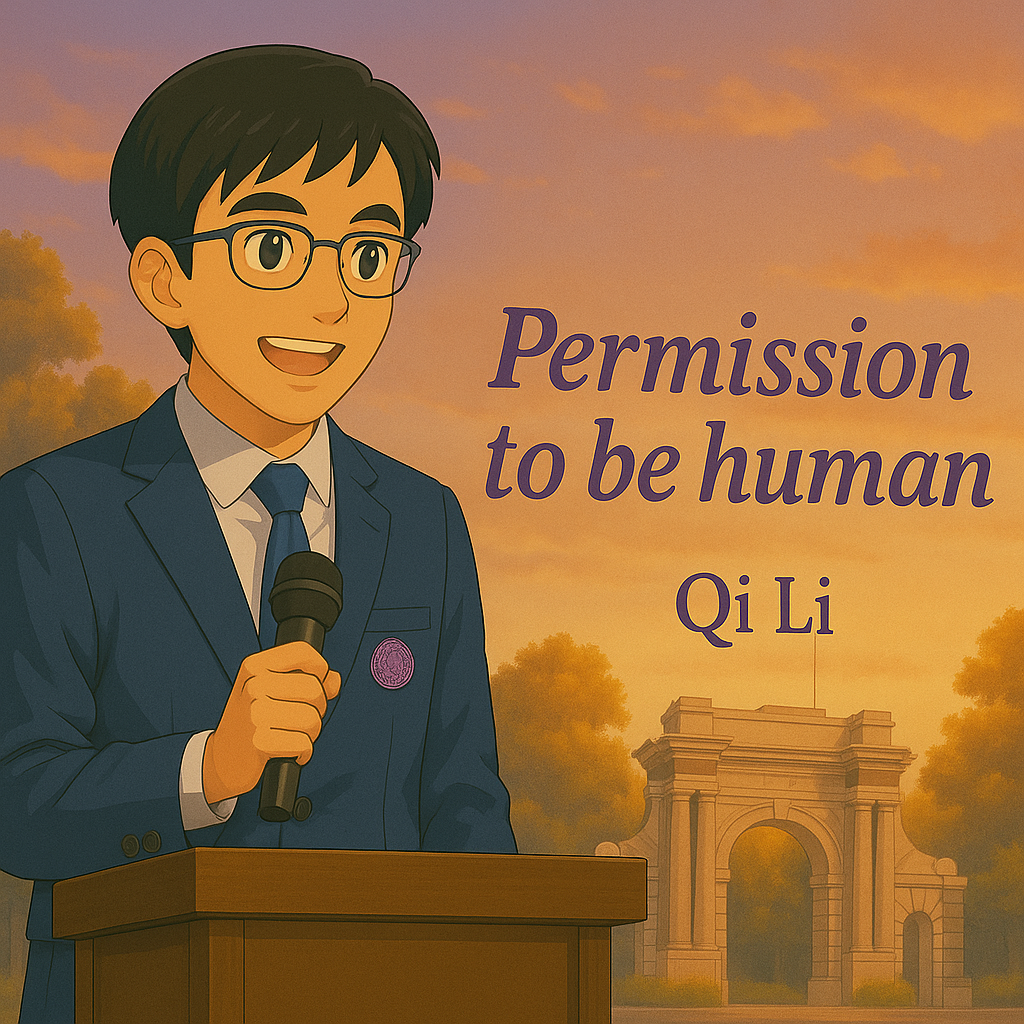
\includegraphics[width=6cm]{../images/LQ.png}}; 
            \end{tikzpicture}
        \end{center}
        }{}
        \vspace{.3cm}
        %%%%%%%%%%%%%%%%%%%%%%%%%%%%%%%%%%%%%%%%%%%%%%%%%%%%
        % YOUR PERSONAL INFROMATION
        \phantomsection{}
        \addcontentsline{toc}{section}{Personal info}
        \section*{\large Personal info}
        \begin{tabularx}{\textwidth}{cY}
            \faGraduationCap{} & Ph.D. Student \\
            \faUniversity{} & Tsinghua University \\
            \faEnvelope{}   & \href{mailto:liq22@tsinghua.org.cn}{liq22@tsinghua.org.cn} \\
            \faMapMarker{}  & Beijing, China \\
            \faIdCard{}     & ORCID: 0000-0001-7105-2818 \\
        \end{tabularx}
        \vspace{.3cm} \\
        \rule{\linewidth}{0.4pt} \\
        %%%%%%%%%%%%%%%%%%%%%%%%%%%%%%%%%%%%%%%%%%%%%%%%%%%%%%%%%
        % YOUR LINKS, YOU MAY ALSO ADD A PERSONAL WEBSITE OR PORTFOLIO
        \phantomsection{}
        \addcontentsline{toc}{section}{Links}
        \section*{\large Links}
        \begin{tabular}{cl}
            \faGithub{}     & \href{https://github.com/liq22}{/liq22} \\
            \faGraduationCap{} & \href{https://scholar.google.com/citations?user=vCabh8oAAAAJ}{Google Scholar} \\
            \faResearchgate{} & \href{https://www.researchgate.net/profile/Qi-Li-155}{ResearchGate} \\
            \faTv{}        & \href{https://space.bilibili.com/1864908149}{Bilibili} \\
        \end{tabular}
        \vspace{10pt} \\
        \rule{\linewidth}{0.4pt} \\
        %%%%%%%%%%%%%%%%%%%%%%%%%%%%%%%%%%%%%%%%%%%%%%%%%%%%%%%%%%%%
        % YOUR SKILLS
        % Add/Remove as seen fit, Icons: https://packages.oth-regensburg.de/ctan/fonts/fontawesome5/doc/fontawesome5.pdf
        \phantomsection{}
        \addcontentsline{toc}{section}{Skills}
        \section*{\large Research \& Skills}
        \begin{tabularx}{\textwidth}{cY}
            \faBrain{}       & Trustworthy AI, Foundation Models, Reliable PHM \\
            \faCode{}        & Python, MATLAB, PyTorch, TensorFlow, Scikit-learn \\
            \faPen*{}        & \LaTeX, Markdown, Academic Writing \\
            \faLanguage{}    & English (CSC: 104/130), Chinese (Native) \\
            \faDesktop{}     & Linux, Windows, HPC Clusters \\
            \faLaptopCode{}  & Jupyter, VS Code, PyCharm \\
            \faToolbox{}     & Git, Docker, MLflow, Weights\&Biases 
        \end{tabularx}
        \vspace{1pt} \\
        \rule{\linewidth}{0.4pt}
        %%%%%%%%%%%%%%%%%%%%%%%%%%%%%%%%%%%%%%%%%%%%%%%%%%%%%%%%%%%%%%%%
        % GRADESCALE (if nesseary, e.g. if you apply abroad, where scales 
        % are different. You should at least provide, what the best possible
        % grade and what the worst possible grade is)
        \vfill
        {\tiny Grade scale: (1) very good $\approx$91\%-100\%, (2) good $\approx$81\%-90\%, (3) satisfactory $\approx$66\%-80\%, (4) sufficient $\approx$50\%-65\%, (5) failed $\approx$0\%-49\%}
    \end{minipage}
}
\hfill
\fcolorbox{red}{mainbg}{%
    \begin{minipage}[t][\dimexpr\textheight-2\fboxrule-2\fboxsep\relax][t]{\dimexpr0.6\textwidth-2\fboxrule-2\fboxsep\relax}
        \color{maintext}
        %%%%%%%%%%%%%%%%%%%%%%%%%%%%%%%%%%%%%%%%%%%%%%%%%%%%%%%%%%
        % RESEARCH EXPERIENCE
        \phantomsection{}
        \addcontentsline{toc}{section}{Research Experience}
        \section*{\scshape\Large Research Experience \rule{\linewidth}{0.4pt}}
%
        {\large \textbf{Yale University}} \\ 
        {{\fontseries{medium}\selectfont Visiting Scholar, Statistics and Data Science}} \\
        {\scshape\fontseries{light}\selectfont\footnotesize Apr 2025 \textendash{} Sep 2025} 
        \begin{itemize}
            \setlength{\itemsep}{-3pt}
            \item Do stuff
            \begin{itemize}
                \item That included Stuff
                \item and more Stuff
            \end{itemize}
            \item Other Task
        \end{itemize}
%
        {\large \textbf{AIR, Tsinghua University}} \\
        {{\fontseries{medium}\selectfont Research Intern}} \\
        {\scshape\fontseries{light}\selectfont\footnotesize Apr 2022 \textendash{} Sep 2022} 
        \begin{itemize}
            \setlength{\itemsep}{-3pt}
            \item Do stuff
            \begin{itemize}
                \item That included Stuff
                \item and more Stuff
            \end{itemize}
            \item Other Task
            \begin{itemize}
                \item That included more Stuff
                \item and other more different Stuff
            \end{itemize}
            \item tellus elementum sagittis vitae et
            \item aliquam sem et tortor consequat
            \item ullamcorper velit sed ullamcorper morbi tincidunt
            \item rhoncus est pellentesque elit ullamcorper dignissim
        \end{itemize}
%
        {\large \textbf{Tsinghua University}}\\
        {{\fontseries{medium}\selectfont Ph.D. Research Assistant}}\\
        {\scshape\fontseries{light}\selectfont\footnotesize Sep 2022 \textendash{} Present} 
        \begin{itemize}
            \setlength{\itemsep}{-4pt}
            \item massa tempor nec feugiat nisl pretium fusce id
        \end{itemize}
        %%%%%%%%%%%%%%%%%%%%%%%%%%%%%%%%%%%%%%%%%%%%%%%%%%%%%%%%%%%
        % EDUCATION
        \phantomsection{}
        \addcontentsline{toc}{section}{Education}
        \section*{\scshape\Large Education \rule{\linewidth}{0.4pt}}
%
        {\large \textbf{Ph.D. Mechanical Engineering, Tsinghua University\\ (Doctoral Degree)}} \\
        {\scshape\fontseries{light}\selectfont\footnotesize Beijing \qquad Sep 2022 \textendash{} Present} \\
        {Supervisor: Prof. Zhaoye Qin} \\[1ex]
        {Research Focus: Trustworthy AI, Foundation Models, PHM} \\[1ex]
        {\footnotesize Publications: 8+ papers in JCR Q1 journals} \\
        {\footnotesize Citations: 600+ (Google Scholar)} \\
        {\footnotesize Awards: Future Scholars Scholarship, CAST Youth Talent Program} \\[2ex]

        {\large \textbf{M.Eng. Control Theory and Control Engineering, Soochow University\\ (Master's Degree)}} \\
        {\scshape\fontseries{light}\selectfont\footnotesize Suzhou \qquad Sep 2019 \textendash{} Jun 2022} \\
        {Supervisors: Prof. Liang Chen \& Prof. Changqing Shen} \\[1ex]
        {Outstanding Graduate, National Scholarship recipient} \\
        {Research: Domain adaptation for fault diagnosis} \\[1ex]
        {\footnotesize Published 3 highly-cited papers in top-tier journals} \\[2ex]

        {\large \textbf{B.Eng. Electrical Engineering, Soochow University}} \\
        {\scshape\fontseries{light}\selectfont\footnotesize Suzhou \qquad Sep 2015 \textendash{} Jun 2019} \\
        {Outstanding Graduate of Soochow University} \\[1ex]
        {Graduate Representative Speaker at Opening Ceremony} \\[1ex]
        {\footnotesize Foundation in electrical systems and control engineering} \\
        % \\
        \vfill%
        {\hfill\small\fontseries{extralight}\selectfont Page \thepage of \pageref{LastPage}\hfill}
    \end{minipage}
}%
\newpage
%%%%%%%%%%%%%%%%%%%%%%%%%%%%%%%%%
% PAGE 2
%%%%%%%%%%%%%%%%%%%%%%%%%%%%%%%%%
\fcolorbox{red}{mainbg}{%
    \begin{minipage}[t][\dimexpr\textheight-2\fboxrule-2\fboxsep\relax][t]{\dimexpr0.6\textwidth-2\fboxrule-2\fboxsep\relax}
        \color{maintext}
        % \vspace{.6cm}
        %%%%%%%%%%%%%%%%%%%%%%%%%%%%%%%%%%%%%%%%%%%%%%%%
        % PUBLICATIONS
        \phantomsection
        \addcontentsline{toc}{section}{Publications}
        \section*{\scshape\Large Selected Publications \rule{\linewidth}{0.4pt}}
        \begin{justify}
        \setlength{\parindent}{0pt}
        {\large \textbf{HSE: A Plug-and-Play Module for Unified Fault Diagnosis}} \\
        {\scshape\fontseries{light}\selectfont\footnotesize Acme Corp \qquad 2017} \\
        \textbf{Qi Li}, Bojian Chen, Qitong Chen, Xuan Li, Zhaoye Qin, Fulei Chu. Propose a novel HSE module that projects heterogeneous signals into a unified signal space for seamless integration with existing fault diagnosis architectures. \\[1ex]
        Skill 1, Skill 2, Skill 3 \\

        {\large \textbf{Lacus laoreet non}} \\
        {\scshape\fontseries{light}\selectfont\footnotesize Acme Corp \qquad 2018} \\
        Pellentesque elit ullamcorper dignissim cras tincidunt. Sit amet commodo nulla facilisi nullam vehicula ipsum. Blandit cursus risus at ultrices mi tempus imperdiet. Lectus sit amet est placerat in egestas erat.\\[1ex]
        Skill 1, Skill 2, Skill 3, \LaTeX \\

        {\large \textbf{Viverra maecenas accumsan lacus}} \\
        {\scshape\fontseries{light}\selectfont\footnotesize Private \qquad 2022 and ongoing} \\
        Quisque non tellus orci ac auctor augue mauris augue neque. Sit amet luctus venenatis lectus magna fringilla urna porttitor rhoncus. Proin nibh nisl condimentum id venenatis a condimentum vitae sapien. \\[1ex]
        Skill 1, Skill 2, Skill 3 \\
        
        {\large \textbf{Ut faucibus pulvinar elementum}} \\
        {\scshape\fontseries{light}\selectfont\footnotesize TU Dresden \qquad 2022} \\
        Proin nibh nisl condimentum id venenatis a condimentum vitae sapien. Amet aliquam id diam maecenas ultricies mi eget. Viverra maecenas accumsan lacus vel facilisis volutpat. \\[1ex]
        Skill 1, Skill 2, Skill 3 \\

        {\large \textbf{Quisque non tellus orci}} \\
        {\scshape\fontseries{light}\selectfont\footnotesize ACME Corp. \qquad 2023} \\
        Viverra maecenas accumsan lacus vel facilisis volutpat. Tortor condimentum lacinia quis vel eros donec ac odio tempor. Ultricies lacus sed turpis tincidunt id aliquet risus. \\[1ex]
        Skill 1, Skill 2, Skill 3 \\
        
        {\large \textbf{Amet consectetur adipiscing elit}} \\
        {\scshape\fontseries{light}\selectfont\footnotesize ACME Corp \qquad 2023} \\
        Eget lorem dolor sed viverra. Eleifend donec pretium vulputate sapien. Pellentesque pulvinar pellentesque habitant morbi tristique senectus et netus et. Augue neque gravida in fermentum et. Ullamcorper velit sed ullamcorper morbi tincidunt ornare massa eget egestas. \\[1ex]
        Skill 1, Skill 2, Skill 3 \\
        
        {\large \textbf{Augue neque gravida in fermentum}} \\
        {\scshape\fontseries{light}\selectfont\footnotesize Sample Uni \qquad 2023} \\
        met aliquam id diam maecenas ultricies mi eget. Viverra maecenas accumsan lacus vel facilisis volutpat. Tortor condimentum lacinia quis vel eros donec ac odio tempor. Ultricies lacus sed turpis tincidunt id aliquet risus. \\[1ex]
        Skill 1, Skill 2, Skill 3, \LaTeX 
        \end{justify}
        \vfill%
        {\hfill\small\fontseries{extralight}\selectfont Page \thepage of \pageref{LastPage}\hfill}
    \end{minipage}
}
\hfill%
\fcolorbox{red}{sidebg}{%
    \begin{minipage}[t][\dimexpr\textheight-2\fboxrule-2\fboxsep\relax][t]{\dimexpr0.4\textwidth-2\fboxrule-2\fboxsep\relax}
        \color{sidetext}
        % \vspace{.5cm}
        %%%%%%%%%%%%%%%%%%%%%%%%%%%%%%%%%%%%%%%%%%%%%%%%%%%%%%%%
        % YOUR NAME AND PREFERED PRONOUS AGAIN AS HEADER
        {\bfseries\scshape\HUGE 李} \\
        {\bfseries\scshape\Huge 奇} \quad {\normalfont\Large Qi Li}
        \vspace{.3cm} \\
        %%%%%%%%%%%%%%%%%%%%%%%%%%%%%%%%%%%%%%%%%%%%%%%%%%%%%%%%%%
        % LANGUAGES
        \phantomsection
        \addcontentsline{toc}{section}{Languages}
        \section*{\large Languages}
        \begin{tabular}{cl}
            \faLanguage{} & Lorem ipsum (Mothertounge) \\
            \faLanguage{} & English (Fluent)
        \end{tabular}
        \vspace{.3cm}
        \\
        \rule{\linewidth}{0.4pt}
        \\
        %%%%%%%%%%%%%%%%%%%%%%%%%%%%%%%%%%%%%%%%%%%%%%%%%%%%%%%%%%%%
        % CERTIFICATES AND AWARDS RECEIVED
        \phantomsection
        \addcontentsline{toc}{section}{Certificates and Prizes}
        \section*{\large Certificates and Prizes}
        \begin{tabularx}{\textwidth}{cY}
            2010 & Etiam tempor orci eu \\
            2010 & Quam nulla porttitor massa \textemdash{} 3\textsuperscript{rd} place \\
            2011 & Quis imperdiet massa tincidunt \textemdash{} 3\textsuperscript{rd} place \\
            2016 & Vestibulum sed arcu non odio euismod \\
            2016 & Non enim praesent elementum facilisis \\
            2016 & Blandit libero volutpat sed cras \\
            2016 & Eget dolor morbi non arcu \\
        \end{tabularx}
        \vspace{.3cm}
        \\
        \rule{\linewidth}{0.4pt}
        \\
        %%%%%%%%%%%%%%%%%%%%%%%%%%%%%%%%%%%%%%%%%%%%
        % HOBBIES
        % Change Icons here https://packages.oth-regensburg.de/ctan/fonts/fontawesome5/doc/fontawesome5.pdf
        \phantomsection
        \addcontentsline{toc}{section}{Hobbies}
        \section*{\large Hobbies}
        \begin{tabularx}{\textwidth}{cY}
            \faCamera{} & Fringilla \\
            \faCogs{} & Id eu nisl nunc mi ipsum \\
        \end{tabularx}
        \vspace{.3cm}
        \\
        \rule{\linewidth}{0.4pt}
    \end{minipage}%
}%
\end{document}
